\vspace{-3cm}\chapter{题目1:创建一个用来表示时间的类}

\section{1.1 题目}
\begin{enumerate}
    \item 创建一个用来存储时间数据的\lstinline{MyTime}类类型,当创建完这个类以后,应该保证下面的测试程序可以运行,且运行的结果如图所示。
    \begin{lstlisting}[
        language = Java,
        caption = {src/hw2/p1/TestTime.java, L5-L31}]
        // Official Test
        MyTime t1 = new MyTime();
        MyTime t2 = new MyTime(2);
        MyTime t3 = new MyTime(21, 34);
        MyTime t4 = new MyTime(12, 25, 42);
        MyTime t5 = new MyTime(t4);

        System.out.println("Constructed with:");
        System.out.println("t1: all arguments defaulted");
        System.out.printf(" %s\n", t1.toUniversalString());
        System.out.printf(" %s\n", t1.toString());
        System.out.println("t2: hour specified; minute and second defaulted");
        System.out.printf(" %s\n", t2.toUniversalString());
        System.out.printf(" %s\n", t2.toString());
        System.out.println("t3: hour and minute specified; second defaulted");
        System.out.printf(" %s\n", t3.toUniversalString());
        System.out.printf(" %s\n", t3.toString());
        System.out.println("t4: hour, minute and second specified");
        System.out.printf(" %s\n", t4.toUniversalString());
        System.out.printf(" %s\n", t4.toString());
        System.out.println("t5: MyTime object t4 specified");
        System.out.printf(" %s\n", t5.toUniversalString());
        System.out.printf(" %s\n", t5.toString());
        // when initialize t6 with invalid values,please output error information
        MyTime t6 = new MyTime(15, 74, 99);
        System.out.println("t6: invalid values");
        System.out.printf("%s\n", t6.toUniversalString());
    \end{lstlisting}
    \begin{figure}[H]
        \centering
        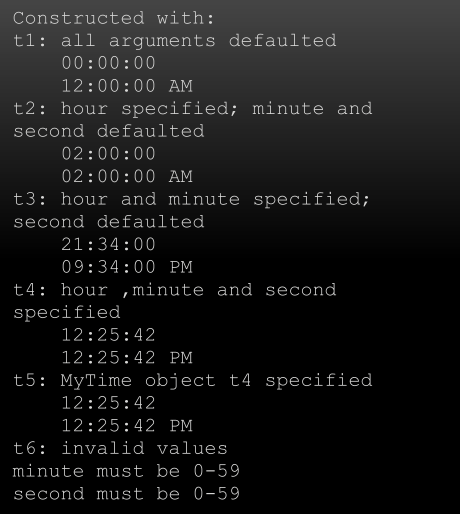
\includegraphics[width = 0.5\textwidth]{../pic/1/1.1.png}
        \caption{运行结果样例}
    \end{figure}
    \item 为\lstinline{MyTime}类增加三个成员方法:
    \begin{lstlisting}[language = Java]
    public void incrementHour();
    public void incrementMinute();
    public void incrementSecond();
    \end{lstlisting}
    每个方法都是在原有的对应数据上进行加1操作,但是一定要注意这种对时间的加1操作的合法性,比如考虑如下场景:\lstinline{MyTime}对象
    中的\lstinline{second}值为59,
    此时调用\lstinline{incrementSecond()}方法之后,\lstinline{second}值会成为0,同时\lstinline{minute}值也应该加1。
    将所有的特殊情况都考虑全面,并给出测试类。
\end{enumerate}


\section{1.2 题目分析}

本题需要对着已有的测试设计编写\lstinline{MyTime}类,并对\lstinline{increment}系列函数编写测试。

\begin{itemize}
    \item \textbf{Field}. 参照代码注释可知,可以定义三个\lstinline{int}变量\lstinline{hour}
        ,\lstinline{minute},\lstinline{second}分别代表小时、分钟、秒钟,24小时制。
    \item \textbf{Constructor Method}. 测试代码中一共出现了5种构造方法
    \begin{itemize}
        \item \lstinline{MyTime()},\lstinline{MyTime(int)},\lstinline{MyTime(int, int)},
        \lstinline{MyTime(int, int, int)};这4种构造方法都是直接将参数赋给类的变量,分别为
        默认、只赋时钟、只赋分钟、全赋值,未赋值的变量默认值为0;
        \item \lstinline{MyTime(MyTime)}这一构造方法是将参量复制给新的对象,即复制参量中的三个变量给新的对象。
        \item 值得注意的是,除了默认的构造方法外,构造方法均可以通过调用其他的构造方法实现,这样可以极大减少代码量,提高代码复用性。
    \end{itemize}
    \item \textbf{Other Method}. 本题目共要求实现编写5个实例化方法
    \begin{itemize}
        \item \lstinline{String toUniversalString()}. 本方法需要先判断\lstinline{this}数据是否合法,根据判断结果返回相应的字符串。
        \begin{enumerate}
            \item 判断\lstinline{this}的数据是否合法,因为错误信息需要检查所有的数据,所以设置一个初值为
                \lstinline{true}的\lstinline{boolean}变量\lstinline{flag},在判断过程中任一的判断错误
                都要将\lstinline{flag}置为\lstinline{false}.
            \item 如果不合法,输出判断过程中生成的错误信息
            \item 如果合法,根据\lstinline{this}的数据输出时间信息。此处需要注意字符串的输出格式:前导空格和Java format中的\lstinline{%02d}. 
        \end{enumerate}
        \item \lstinline{String toString()}. 本方法只需返回12小时制的时间字符串,所以只需注意\lstinline{hour}数据的处理和格式问题。
        \begin{enumerate}
            \item 参看测试代码可知,如果\lstinline{hour%12}为0,我们需要输出为12点,其他情况取余即可
            \item 格式问题可以参照上一个方法中的第三条,并在最后附上\lstinline{AM}/\lstinline{PM}
        \end{enumerate}
        \item \lstinline{increment}系列方法. 这几个方法逻辑基本类似,都是判断数据\lstinline{++}后是否超过上界,如果越界了需要将该数据置为0,
        并将更高级的单位数据\lstinline{++}。
        \begin{itemize}
            \item 基于这种\lstinline{++}操作的传递性,我们可以通过调用上一级单位的\lstinline{increment}方法简化我们的代码逻辑。
        \end{itemize}
    \end{itemize}
    \item \textbf{Test for Increment}. 测试代码只需确定每个\lstinline{increment}函数都正确无误,并测试其易错的进位即可,根据这个思路设计
        \lstinline{01:02:03}和\lstinline{23:59:59}. 
    两个数据。
    
\end{itemize}

\section{1.3 结果展示}

\begin{figure}[H]
    \centering
    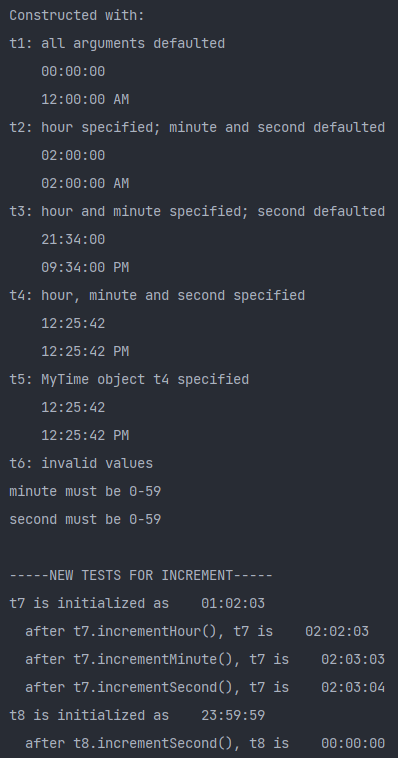
\includegraphics[width = 0.5\textwidth]{../pic/1/1.4.png}
    \caption{运行结果}
\end{figure}

\section{1.4 主干代码}

\begin{lstlisting}[
    language = Java,
    caption = {MyTime.java L8-L87}]
    public class MyTime {
    int hour;
    int minute;
    int second;

    MyTime() {
        hour = 0;
        minute = 0;
        second = 0;
    }

    MyTime(int h) {
        this();
        hour = h;
    }

    public MyTime(int h, int m) {
        this(h);
        minute = m;
    }

    public MyTime(int h, int m, int s) {
        this(h, m);
        second = s;
    }

    public MyTime(MyTime t4) {
        this(t4.hour, t4.minute, t4.second);
    }

    boolean ValidJudge(int num) {
        return num < 0 || num >= 60;
    }

    public String toUniversalString() {
        boolean flag = true;
        String s = "";

        if (ValidJudge(hour)) {
            flag = false;
            s += "hour must be 0-23\n";
        }
        if (ValidJudge(minute)) {
            flag = false;
            s += "minute must be 0-59\n";
        }
        if (ValidJudge(second)) {
            flag = false;
            s += "second must be 0-59\n";
        }
        if (flag) return String.format("   %02d:%02d:%02d", hour, minute, second);
        else return s;
    }

    @Override
    public String toString() {
        String s;
        s = (hour % 12 == 0) ? String.format("   %02d:%02d:%02d ", 12, minute, second) :
                String.format("   %02d:%02d:%02d ", hour % 12, minute, second);
        s += (hour < 12) ? "AM" : "PM";
        return s;
    }

    public void incrementHour() {
        if (++hour >= 24) hour = 0;
    }

    public void incrementMinute() {
        if (++minute >= 60) {
            minute = 0;
            incrementHour();
        }
    }

    public void incrementSecond() {
        if (++second >= 60) {
            second = 0;
            incrementMinute();
        }
    }
\end{lstlisting}

\begin{lstlisting}[
    language = Java,
    caption = {TestTime.java L33-L46}]
    // My Test for new increment methods
        System.out.println("-----NEW TESTS FOR INCREMENT-----");
        MyTime t7 = new MyTime(1,2,3);
        System.out.printf("t7 is initialized as %s\n",t7.toUniversalString());
        t7.incrementHour();
        System.out.printf("  after t7.incrementHour(), t7 is %s\n", t7.toUniversalString());
        t7.incrementMinute();
        System.out.printf("  after t7.incrementMinute(), t7 is %s\n", t7.toUniversalString());
        t7.incrementSecond();
        System.out.printf("  after t7.incrementSecond(), t7 is %s\n", t7.toUniversalString());
        MyTime t8 = new MyTime(23, 59, 59);
        System.out.printf("t8 is initialized as %s\n",t8.toUniversalString());
        t8.incrementSecond();
        System.out.printf("  after t8.incrementSecond(), t8 is %s\n", t8.toUniversalString());
\end{lstlisting}

\section{1.5 总结与收获}

本题目较为简单,但其中蕴含的方法间互相调用以提高代码复用率的思想让我收益良多。

本题中的输出涉及大量关于细节,包括:如何让代码的逻辑更舒服更“美”、java字符串的format形式等等,这些细节虽然加起来不到三五行,却占据了我
50\%以上的时间,尤其是对代码逻辑的优化和打磨需要反复斟酌。

% 1、题目
% 2、数据设计
% 3、算法设计
% 4、主干代码说明
% 5、运行结果展示
% 6、总结和收获